%File: anonymous-submission-latex-2025.tex
\documentclass[letterpaper]{article} % DO NOT CHANGE THIS
\usepackage[submission]{aaai25}  % DO NOT CHANGE THIS
\usepackage{times}  % DO NOT CHANGE THIS
\usepackage{helvet}  % DO NOT CHANGE THIS
\usepackage{courier}  % DO NOT CHANGE THIS
\usepackage[hyphens]{url}  % DO NOT CHANGE THIS
\usepackage{graphicx} % DO NOT CHANGE THIS
\urlstyle{rm} % DO NOT CHANGE THIS
\def\UrlFont{\rm}  % DO NOT CHANGE THIS
\usepackage{natbib}  % DO NOT CHANGE THIS AND DO NOT ADD ANY OPTIONS TO IT
\usepackage{caption} % DO NOT CHANGE THIS AND DO NOT ADD ANY OPTIONS TO IT
\frenchspacing  % DO NOT CHANGE THIS
\setlength{\pdfpagewidth}{8.5in} % DO NOT CHANGE THIS
\setlength{\pdfpageheight}{11in} % DO NOT CHANGE THIS
\usepackage{algorithm}
\usepackage{algorithmic}

%
% These are are recommended to typeset listings but not required. See the subsubsection on listing. Remove this block if you don't have listings in your paper.
\usepackage{newfloat}
\usepackage{listings}
\DeclareCaptionStyle{ruled}{labelfont=normalfont,labelsep=colon,strut=off} % DO NOT CHANGE THIS
\lstset{%
	basicstyle={\footnotesize\ttfamily},% footnotesize acceptable for monospace
	numbers=left,numberstyle=\footnotesize,xleftmargin=2em,% show line numbers, remove this entire line if you don't want the numbers.
	aboveskip=0pt,belowskip=0pt,%
	showstringspaces=false,tabsize=2,breaklines=true}
\floatstyle{ruled}
\newfloat{listing}{tb}{lst}{}
\floatname{listing}{Listing}
%
% Keep the \pdfinfo as shown here. There's no need
% for you to add the /Title and /Author tags.
\pdfinfo{
/TemplateVersion (2025.1)
}

% DISALLOWED PACKAGES
\usepackage{amsmath,amsthm,amsfonts,amssymb}
\newtheorem{theorem}{Theorem}
\newtheorem{lemma}[theorem]{Lemma}
\newtheorem{asmp}[theorem]{Assumption}
\newtheorem{example}[theorem]{Example}
\newtheorem{question}[theorem]{Question}
\newtheorem{proposition}[theorem]{Proposition}
\newtheorem{corollary}[theorem]{Corollary}
\newtheorem{property}[theorem]{Property}
\theoremstyle{definition}
\newtheorem{definition}[theorem]{Definition}
\theoremstyle{remark}
\newtheorem{remark}[theorem]{Remark}

\usepackage{stackengine}
\def\delequal{\mathrel{\ensurestackMath{\stackon[1pt]{=}{\scriptstyle\Delta}}}}

\usepackage{tikz}
\usetikzlibrary{arrows, fit, backgrounds, positioning} 
\usepackage{tcolorbox}
% \usepackage{authblk} -- This package is specifically forbidden
% \usepackage{balance} -- This package is specifically forbidden
% \usepackage{color (if used in text)
% \usepackage{CJK} -- This package is specifically forbidden
% \usepackage{float} -- This package is specifically forbidden
% \usepackage{flushend} -- This package is specifically forbidden
% \usepackage{fontenc} -- This package is specifically forbidden
% \usepackage{fullpage} -- This package is specifically forbidden
% \usepackage{geometry} -- This package is specifically forbidden
% \usepackage{grffile} -- This package is specifically forbidden
% \usepackage{hyperref} -- This package is specifically forbidden
% \usepackage{navigator} -- This package is specifically forbidden
% (or any other package that embeds links such as navigator or hyperref)
% \indentfirst} -- This package is specifically forbidden
% \layout} -- This package is specifically forbidden
% \multicol} -- This package is specifically forbidden
% \nameref} -- This package is specifically forbidden
% \usepackage{savetrees} -- This package is specifically forbidden
% \usepackage{setspace} -- This package is specifically forbidden
% \usepackage{stfloats} -- This package is specifically forbidden
% \usepackage{tabu} -- This package is specifically forbidden
% \usepackage{titlesec} -- This package is specifically forbidden
% \usepackage{tocbibind} -- This package is specifically forbidden
% \usepackage{ulem} -- This package is specifically forbidden
% \usepackage{wrapfig} -- This package is specifically forbidden
% DISALLOWED COMMANDS
% \nocopyright -- Your paper will not be published if you use this command
% \addtolength -- This command may not be used
% \balance -- This command may not be used
% \baselinestretch -- Your paper will not be published if you use this command
% \clearpage -- No page breaks of any kind may be used for the final version of your paper
% \columnsep -- This command may not be used
% \newpage -- No page breaks of any kind may be used for the final version of your paper
% \pagebreak -- No page breaks of any kind may be used for the final version of your paperr
% \pagestyle -- This command may not be used
% \tiny -- This is not an acceptable font size.
% \vspace{- -- No negative value may be used in proximity of a caption, figure, table, section, subsection, subsubsection, or reference
% \vskip{- -- No negative value may be used to alter spacing above or below a caption, figure, table, section, subsection, subsubsection, or reference

\setcounter{secnumdepth}{0} %May be changed to 1 or 2 if section numbers are desired.

% The file aaai25.sty is the style file for AAAI Press
% proceedings, working notes, and technical reports.
%

% Title

% Your title must be in mixed case, not sentence case.
% That means all verbs (including short verbs like be, is, using,and go),
% nouns, adverbs, adjectives should be capitalized, including both words in hyphenated terms, while
% articles, conjunctions, and prepositions are lower case unless they
% directly follow a colon or long dash
\title{A Novel Information Fusion Framework Based on a Simple Stochastic Aggregation Operator with Applications in Decision-Making}

% REMOVE THIS: bibentry
% This is only needed to show inline citations in the guidelines document. You should not need it and can safely delete it.
\usepackage{bibentry}
% END REMOVE bibentry

\begin{document}

\maketitle

\begin{abstract}
Information fusion plays a critical role in decision-making, particularly in complex scenarios. When formalizing information fusion, information is commonly represented as probability distributions, with the Bayesian framework serving as a powerful and predominant method. However, despite its theoretical strength, Bayesian methods often involve intricate computations, even when using exponential family priors, which can limit their practicality in certain decision contexts. This paper introduces a novel information fusion framework based on a simple stochastic aggregation operator. Our key insight lies in customizing appropriate measurable spaces for specific decision-making scenarios, a crucial distinction from the Bayesian approach that allows for more intuitive and computationally efficient information fusion. We demonstrate this customization in various settings, including counterfactual-based personalization and Direct Preference Optimization (DPO). The framework's core is a mathematically simple yet rigorous aggregation operator with elegant properties, including an Abelian group structure. While complementing rather than replacing Bayesian methods, our framework presents a distinctive alternative characterized by its mathematical simplicity and intuitive nature, potentially broadening the toolkit for information fusion in decision-making contexts.

\end{abstract}


\section{Introduction}


In decision-making, representing information with probability distributions is essential. Clemen and Winkler\cite{clemen2007aggregating} highlight the integration challenge of different information sources, such as scientific models and forecasting methods, especially when data is scarce. Aggregating these distributions improves our understanding of the available knowledge and uncertainties, aiding in informed decision-making.  The aggregation of probabilities typically follows either mathematical or behavioral methods. Mathematical approaches combine individual probability distributions into a unified whole. These methods, particularly Bayesian ones, are noted for their systematic updating of probabilities with new data \cite{jouini1996copula,sklar1996random}. In contrast, behavioral methods involve creating a consensus among experts through interaction \cite{ferrell1985combining}. While they might be less exact than mathematical methods, they effectively harness collective expertise for better decision-making, filtering out repetitive or less relevant information. 

In this paper, we propose a novel approach to information fusion that combines mathematical elegance with practical applicability. Our method introduces a simple stochastic aggregation operator that forms the foundation of a highly interpretable and intuitive framework for combining probabilistic information.

The key innovation of our approach lies in the careful selection of appropriate measurable spaces tailored to specific decision-making contexts. This crucial step allows us to represent diverse types of information as probability distributions within a unified framework, enabling straightforward aggregation through our proposed operator. Our framework offers several notable advantages:

\begin{enumerate}
    \item \textbf{Simplicity and Interpretability}: The core aggregation operation is mathematically simple and intuitively interpretable, facilitating its adoption and understanding in various decision-making scenarios.
    
    \item \textbf{Mathematical Elegance}: Our framework exhibits beautiful mathematical properties, including an Abelian group structure. This elegance provides a solid theoretical foundation while maintaining simplicity.
    
\end{enumerate}

We demonstrate the utility of our framework through applications in diverse fields, including: 1) Personalized incentive optimization; 2) Aggregation of multiple expert predictions; 3) DPO in alignment of large language models. These case studies illustrate how our approach can provide new insights and potentially improve decision-making processes across various domains. While our framework does not aim to replace established Bayesian methods, it offers a complementary perspective that may be particularly valuable in scenarios where computational simplicity and intuitive interpretability are paramount.

The remainder of this paper is organized as follows: Section 2 provides preliminaries on stochastic aggregation. Section 3 introduces our core stochastic aggregation operation. Section 4 explores the Abelian group structure of our framework. Section 5 discusses adaptations and extensions of our framework. Section 6 demonstrates an application in Direct Preference Optimization. Finally, Section 7 concludes the paper with a discussion of implications and future research directions.


\section{Preliminaries on Stochastic Aggregation}

Traditional aggregation methods in statistics, such as mean, median, maximum, and minimum, typically involve simple mathematical operations applied either to different instances of a single variable or across multiple variables. These methods, while effective for summarizing central tendencies or range of data, do not directly address the aggregation of entire probability distributions. 

 
The Bayesian paradigm, directly operates on distributions, presents a powerful framework for the fusion of information from various sources (See e.g. \cite{clemen2007aggregating, sklar1996random}). It is fundamentally based on Bayes' theorem, which offers a mechanism to update a probability distribution by combining prior knowledge with new evidence. Given a set of information \( e_1, e_2, \ldots, e_n \) regarding an event or quantity of interest \(U\), the updated probability distribution \( p^* \) can be calculated using the following formula:
\begin{align}
\label{agg:bayes}
    p^* \delequal p(u | e_1, \ldots, e_n) \propto p(u) L(e_1, \ldots, e_n | u),
\end{align}
where \( L \) represents the likelihood function associated with the observed information, and the symbol $\propto$ denotes proportionality. This principle can be applied to aggregate any type of information represented by probability distributions. 

However, the computation of $p^*$ is often very challenging, particularly in complex scenarios with intricate dependency structures. The most common approach to simplify this calculation is the use of exponential family prior distributions. However, this method has several drawbacks, including limited flexibility, interpretability issues, and lack of robustness. An alternative and flexible approach involves utilizing statistical tools such as Copulas.
 % $p^*$ 的计算通常是非常困难的, 最常见简化计算 $p^*$ 方法是使用指数族 prior distribution,  这种方法会有灵活性受限, 可解释性问题, 不够robust诸多缺点. 另外一种更灵活的方法是使用统计学工具 Copula.
Copulas are used to describe/model the dependence (inter-correlation) between random variables, which have been used widely in quantitative finance. Sklar's theorem states that any multivariate joint distribution can be written in terms of univariate marginal distribution functions and a copula which describes the dependence structure between the variables.
\begin{theorem}[Sklar's Theorem \cite{renyi1959measures}]
    Let \( H \) be a joint distribution function of random variables with marginal distribution functions \( F_1, F_2, \ldots, F_n \). Then there exists a copula \( C \) such that for all \( u_1, u_2, \ldots, u_n \),
    \begin{equation*}
        H(u_1, u_2, \ldots, u_n) = C(F_1(u_1), \ldots, F_n(u_n)).
    \end{equation*}
    If \( H \) has a density \( h \), and the marginals \( F_i \) have densities \( f_i \), then 
    \begin{equation*}
        h(u_1, \ldots, u_n) = c(F_1(u_1), \ldots, F_n(u_n)) \cdot f_1(u_1)  \cdot \ldots \cdot f_d(u_n),
    \end{equation*}
    where \( c \) is the density of \( C \). If all marginals \( F_i \) are continuous, then \( C \) is unique.
\end{theorem}
It is proposed that by using copula to describe dependence structure, the posterior probability in Eq. \eqref{agg:bayes} can be simplified to:
\begin{align}
\label{agg:bayes_c}
   p^* \propto c[1-F_1(u), \ldots, 1-F_n(u)] \prod_{i=1}^{n} f_i(u),  
\end{align}
where 
\begin{align}
\label{asp:one_info}
    f_i(u) = p(u | e_i)
\end{align}
represents the posterior probability given the information \( e_i \) \cite{jouini1996copula}, which implicitly assumes that there exists a posterior $f_i$ given the prior $p(u)$ represents the information $e_i$ for any $i$. Hence, we refer this as to the ``prior-dependent'' distribution representation for information. The underlying logic of this method provides a mathematical framework for fusing prior information and multiple pieces of evidence. In this framework, each piece of evidence generates a distribution, and the fused information is constructed as a distribution that incorporates all these individual distributions. Consequently, it can be argued that the copula-based Bayesian method is mathematically founded on the principle of \emph{Stochastic Aggregation for Distributions}. 


However, the key formula \eqref{agg:bayes_c} involves concepts and computations of considerable complexity. In the following sections, we introduce an intuitive information fusion framework that offers significant mathematical simplicity.



\section{The Stochastic Aggregation Operation}


When utilizing probability distributions to represent information, the fusion of information is formalized through the stochastic aggregation of probability distributions. This naturally leads to a fundamental question: ``What is the simplest mathematical framework for aggregating two distributions?'' In response, we propose the following mathematical operator:

% \begin{definition}[Stochastic Aggregation for Distributions]
% Let \( P_1 \) and \( P_2 \) be two probability distributions. The Stochastic Aggregation of \( P_1 \) and \( P_2 \), denoted as \( P_1 \odot P_2 \), is defined as a new probability distribution \( P \) whose probability density or mass function \( p(x) \) for a given outcome \( x \) is given by:
% \begin{equation}
%     p(x) \propto p_1(x) p_2(x)
% \end{equation}
% where \( p_1(x) \) and \( p_2(x) \) are the probability densities or mass functions of \( P_1 \) and \( P_2 \) respectively.
% \end{definition}

% Note that the symbol \( \propto \) denotes proportionality, implying that the right-hand side should be normalized to ensure \( p(x) \) is a valid probability distribution.


\begin{definition}[Stochastic Product Operator for Probability Measures]
Let $(\Omega, \mathcal{F})$ be a measurable space, and let $P_1$ and $P_2$ be probability measures on $(\Omega, \mathcal{F})$. The Stochastic Product of $P_1$ and $P_2$, denoted as $P_1 \odot P_2$, is defined as a new probability measure $P$ on $(\Omega, \mathcal{F})$ such that:
\begin{equation}
    P(A) \propto P_1(A)P_2(A)
\end{equation}
, for any atom event $A$.  where the symbol $\propto$ denotes proportionality, implying that the right-hand side should be normalized to ensure $P$ is a valid probability measure.
\end{definition}


This stochastic product operator shares some similarities with the Product of Experts model introduced by \citet{hinton2002training}, although our formulation and application differ in several key aspects. While Hinton's work focuses on machine learning model construction, our operator is formulated in a more general measure-theoretic framework for probability fusion. 

\begin{example}[Stochastic Aggregation for Probability Distributions]
Consider a set of $K$ independent standard normal distributions, each denoted by $\mathcal{N}(0, 1)$. Applying the Stochastic Product Operator, we derive an aggregated distribution $\mathcal{N}^*$ as follows:

\begin{equation}
\mathcal{N}^* = \underbrace{\mathcal{N}(0, 1) \odot  \cdots \odot \mathcal{N}(0, 1)}_{\text{$K$ times}}
\end{equation}

where $\odot$ denotes the Stochastic Product Operator. 

It can be demonstrated that the resulting distribution $\mathcal{N}^*$ is a normal distribution with mean 0 and variance $\frac{1}{K}$, expressed as $\mathcal{N}(0, \frac{1}{K})$. This result yields two significant interpretations:

\begin{enumerate}
    \item \textbf{Information Fusion:} The combination of $K$ independent opinions, each represented by $\mathcal{N}(0, 1)$, results in a collective opinion with a reduced variance of $\frac{1}{K}$. This variance reduction can be interpreted as an increase in the precision of the aggregated information.
    
    \item \textbf{Sampling Theory Parallel:} This result aligns with a fundamental concept in sampling theory. If one were to draw $K$ independent samples from $\mathcal{N}(0, 1)$ and compute their arithmetic mean, the distribution of this sample mean would follow $\mathcal{N}(0, \frac{1}{K})$. This parallel highlights the connection between our aggregation method and established statistical principles.
\end{enumerate}

\end{example}

The concept of stochastic aggregation naturally extends from probability distributions to random variables. This extension is formalized in the following definition:
\begin{definition}[Stochastic Aggregation for Random Variables]
\label{def:agg_rv}
Let $X_1$ and $X_2$ be two random variables defined on the same probability space $(\Omega, \mathcal{F}, P)$. The Stochastic Aggregation of $X_1$ and $X_2$, denoted as $X_1 \odot X_2$, is defined as a new random variable $X$ whose probability function $p_X$ is given by the Stochastic Product of the probability functions of $X_1$ and $X_2$. Specifically, we have:
\begin{equation}
\label{eq:proto}
p_X(x) \propto p_1(x)p_2(x)
\end{equation}
where $p_1$ and $p_2$ are the probability functions of $X_1$ and $X_2$, respectively. Here, $p(x)$ represents the probability density function for continuous random variables or the probability mass function for discrete random variables.
\end{definition}

% Eq. \eqref{eq:proto} 和 Eq. \eqref{agg:bayes_c} 有两个主要区别, 第一个就是不涉及到 prior 信息, 第二个就是 copula function 有关的 density 是常数, 意味着证据信息的某种 conceptual independence. 所以我们的信息融合方法, 可以说是一种最符合直觉, 数学最简单的方式. 
The stochastic aggregation operation defined in Eq. \eqref{eq:proto} exhibits two key differences from Eq. \eqref{agg:bayes_c}. First, it does not involve prior information. Second, the copula-related density is constant, implying a form of conceptual independence among the pieces of evidence. Consequently, our information fusion method can be considered the most intuitive and mathematically simplest approach available. 


% 这种方法的优势: 数学性质特别好和可解释性非常强. 
This approach offers two significant advantages: excellent mathematical properties and strong interpretability. The mathematical elegance of this method is evident in its simplicity and the well-defined properties of the stochastic product operator. Furthermore, the straightforward nature of the aggregation process enhances its interpretability, allowing for clear and intuitive understanding of how different pieces of information are combined, which is particularly valuable in decision-making contexts. 


\section{The Abelian Group Structure}
A fundamental question arises regarding our proposed simple information fusion framework: In which practical decision-making scenarios can this framework be effectively applied, and through what methods can its advantages be fully leveraged?
To address this question, we turn our attention to a critical concern in contemporary internet platforms: the optimization of user retention within budget constraints through various incentive strategies. Personalized incentives based on causal relationships have emerged as a prevalent approach to address this challenge \cite{ai2022lbcf}.  A simplified illustrative example would be:

\begin{example}[The Personalized Decision-making Setting]
\label{eg:incentive}
Consider a causal model tailored for personalized incentives, encompassing observable variables: $S$, $\mathbf{X}$, $T$, and $Y$, as depicted in the causal diagram (Figure \ref{fig:incentive}). The causal mechanisms for each participant $u$ are described below:
\begin{enumerate}
    \item $S$:  Assigns users to one of three experiment groups. The random group ($S=0$) receives incentives based purely on chance; the pure strategy group ($S=1$) has incentives tailored according to specific user characteristics; and the mixed strategy group ($S=2$) combines random allocation with user-specific strategies.
    \item $\mathbf{X}$: Denotes the pre-treatment features of the user that influence both the treatment and outcome. This includes demographic details, historical engagement levels, and other relevant factors. 
    \item $T$: A binary incentive treatment variable. For users in the random group ($S=0$), this decision is made with uniform probability; For users in the pure strategy group ($S=1$), the incentive is a deterministic function of the pre-treatment features; In the mixed strategy group ($S=2$), the decision is influenced by the user's features but retains some randomness.
    \item $Y$: The outcome variable of the user's reaction to the incentive, e.g. conversion, purchase or retention.
\end{enumerate}
\begin{figure}[http]
\centering
    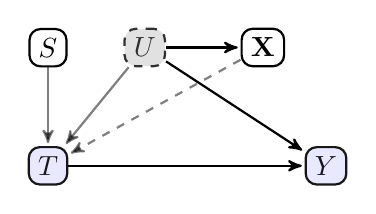
\begin{tikzpicture}[->, >=stealth', shorten >=1pt, auto, thick, node distance=1.5cm, main node/.style={rectangle, rounded corners, draw}]
    \node[main node] (T) {$S$};
    \node[main node, opacity=0.9, fill=blue!10] (A) [below of=T] {$T$};
    \node[main node, opacity=0.9, fill=blue!10] (Y) [right=3cm of A] {$Y$}; % Increase distance between A and Y
    \node[main node, dashed, opacity=0.8, fill=gray!30] (Z) [above right=1cm and 0.7cm of A] {$U$}; % Position Z above and to the left of A
    \node[main node] (X) [right of=Z] {$\mathbf{X}$};
    \path[every node/.style={font=\sffamily\small}]
        (T) edge [opacity=0.5] node {} (A)
        (Z) edge [opacity=0.5] node {} (A)
        (Z) edge node {} (X)
        (Z) edge node {} (Y)
        (A) edge node {} (Y)
        (X) edge [dashed, opacity=0.5] node [midway, above, sloped] {} (A); % Dashed edge from X to A
    \end{tikzpicture}
    \caption{Causal Model for Personalized Incentives: This diagram illustrates the causal relationships among group assignment $S$, incentive treatment $T$, pre-treatment features $\mathbf{X}$, and the outcome variable $Y$. The model integrates a unit representation $U$, capturing all relevant endogenous information (excluding $T$) that determines the Layer valuations regarding to $(T, Y)$.}
\label{fig:incentive}
\end{figure}
\end{example}

% 在这个场景下, 我们把平台中的全部用户组成总体当成一个可测空间 $\mathcal{U}$, 任何一个随机变量 that select an individual 都会有一个对应的概率分布, 信息就用这些概率分布表示, for example evidence/observation $Y=y$, 无论哪个框架因果建模 PO/SCM/DiscoSCM ,  evidence abduction 得到的是  $\mathcal{U}$ 上一个分布, denoted as $U(y)$. 更进一步, 多个 evidence 怎么办呢?  例如 for a subpopulation with homogeneity across individuals, observations $y_1, ..., y_n$ (i.i.d samples) 的信息融合起来其实就是每个 evidence 得到的信息进行融合. i.e. 
% $$U(y_1, ..., y_n) = U(y_1) \odot \cdots U(y_n)$$
In this scenario, we conceptualize the entire user base of the platform as a measurable space $\mathcal{U}$. Any random variable that selects an individual from this space corresponds to a probability distribution. We represent information using these probability distributions. For instance, consider the evidence or observation $Y=y$. Regardless of the causal modeling framework employed (Potential Outcomes\cite{rubin1974estimating}, Structural Causal Models \cite{pearl2009causality}, or Distribution-consistency Structural Causal Models \cite{gong2024distribution}), the process of evidence abduction yields a distribution over $\mathcal{U}$, which we denote as $U(y)$.

This approach naturally extends to multiple pieces of evidence, addressing scenarios that pose challenges for mainstream causal frameworks. Consider a subpopulation exhibiting homogeneity across individuals, where we have observations $y_1, ..., y_n$.The homogeneity assumption allows us to treat these samples as independent and identically distributed (i.i.d.). The fusion of information from these observations can be conceptualized as the aggregation of information obtained from each individual piece of evidence. Mathematically, this can be expressed as:
$$U(y_1, ..., y_n) = U(y_1) \odot \cdots \odot U(y_n)$$
where $\odot$ represents our stochastic product operator for information fusion. This formulation elegantly captures the process of combining multiple observations within our proposed framework. It demonstrates how our simple information fusion method can be applied to aggregate evidence in a principled manner. 

% 这个例子展示我们信息融合框架的基本逻辑, 根据某个具体场景设计一个合适可测空间, 并通过一些特定的步骤, 将信息表示成这个可测空间中的概率分布, 然后使用 Stochastic Product Operator 来融合这些概率分布. 接下来我们进一步形式化的说明该 Decison-making setting 下这个信息融合框架的优美性质。

This example illustrates the fundamental logic of our information fusion framework. The process involves designing an appropriate measurable space for a specific scenario, representing information as probability distributions within this space, and then employing the Stochastic Product Operator to fuse these distributions. We will now formalize the elegant properties of this information fusion framework in the context of our decision-making setting.

\begin{definition}[Information Fusion]
\label{def:infoagg}
Let \( S_1 \) and \( S_2 \) be two unit selection variable of the population $\mathcal{U}$. The Information fusion of \( S_1 \) and \( S_2 \), denoted as \( S_1 \odot S_2 \), is defined as a unit selection variable \( S \) whose distribution $p(u)$ satisfies:
\begin{equation}
\label{eq:infoagg}
    p(u) \propto p_{1}(u) p_{2}(u)
\end{equation}
where $p_{1}(u)$ and $p_{2}(u)$ are the respective distributions of $S_1$ and $S_2$. \footnote{These distributions represent posteriors obtained by updating a uniform prior, such as distributions resulting from evidence abduction.}
\end{definition}

The Information Fusion operation, denoted as $\odot$, inherits several desirable properties from the Stochastic Product Operator. These properties collectively form an algebraic structure known as an Abelian Group. We formally define these properties below:

\begin{property}[Commutativity]
For all unit selection variables $S_1$ and $S_2$ in the population $\mathcal{U}$, the operation $\odot$ is commutative if:
\begin{equation}
    S_1 \odot S_2 = S_2 \odot S_1
\end{equation}
\end{property}

\begin{property}[Associativity]
For all unit selection variables $S_1$, $S_2$, and $S_3$ in the population $\mathcal{U}$, the operation $\odot$ is associative if:
\begin{equation}
    (S_1 \odot S_2) \odot S_3 = S_1 \odot (S_2 \odot S_3)
\end{equation}
\end{property}

\begin{property}[Identity Element]
\label{property:identity}
There exists an element $U$, such that for any unit selection variable $S$ in the population $\mathcal{U}$:
\begin{equation}
    S \odot U = S
\end{equation}
\end{property}

\begin{property}[Inverse Element]
\label{property:inverse}
For every unit selection variable $S$ with non-zero probability on every unit $u \in \mathcal{U}$\footnote{For unit selection variables with zero probability on some units, special techniques are required.}, there exists a unique inverse $S^*$, such that:
\begin{equation}
    S \odot S^* = U
\end{equation}
\end{property}

\begin{theorem}
The Information Fusion operation $\odot$ forms an Abelian Group on the set of unit selection variables of the population $\mathcal{U}$.
\end{theorem}

\begin{proof}
Commutativity and associativity are directly evident from the operation's definition in Eq. \eqref{eq:infoagg}, where $S_1 \odot S_2 = S_2 \odot S_1$ and $(S_1 \odot S_2) \odot S_3 = S_1 \odot (S_2 \odot S_3)$, due to the commutative and associative nature of multiplication in probability densities.

The uniform distribution over $\mathcal{U}$ acts as the identity element, as $S \odot U = S$ for any unit selection variable $S$, maintaining the original probability density unchanged.

Lastly, the inverse element for each unit selection variable $S$, denoted as $S^*$, can be constructed using inverse probabilities as weights. For a unit selection variable $S$ with probability density $p(u)$, its inverse $S^*$ has a probability density proportional to $\frac{1}{p(u)}$. This ensures that $S \odot S^*$ aligns with the uniform distribution, thus fulfilling the requirement for an inverse element.

Therefore, the Information Fusion operation $\odot$ satisfies all the properties of an Abelian Group.
\end{proof}

This group structure endows the operation with several significant advantages:

\begin{enumerate}
    \item \textbf{Flexible Information Combination}: The commutative and associative properties allow for the fusion of information from multiple sources in any order, providing flexibility in the aggregation process.
    
    \item \textbf{Consistency in Aggregation}: The identity element ensures that combining a piece of information with no information (represented by the uniform distribution) does not alter the original information.
    
    \item \textbf{Information Reversal}: The existence of inverse elements allows for the theoretical "removal" of a piece of information from an aggregated whole, which can be crucial in certain analytical scenarios.
    
    \item \textbf{Mathematical Rigor}: The group structure provides a solid mathematical foundation for operations on information, allowing for the application of well-established algebraic techniques in information processing.
\end{enumerate}

These properties collectively establish a robust framework for information fusion in our decision-making context, particularly in scenarios involving counterfactual-based personalized incentives as described in Example \ref{eg:incentive}.

\section{Adaptation of the Information Fusion Framework}

Our proposed information fusion framework, initially introduced for specific decision-making scenarios, shows promising potential for adaptation to a wider range of information types and probability distributions. While acknowledging potential limitations, we explore how this framework can be extended to accommodate diverse forms of information, thereby possibly enhancing its versatility and applicability.
One significant extension is the incorporation of set-based information. This adaptation allows us to integrate subset information into our fusion framework, potentially broadening its scope. To formalize this concept, we introduce the notion of Set Information Fusion:
\begin{definition}[Set Information Fusion]
Let $\mathcal{U}$ be the population space, and consider a set $A \subseteq \mathcal{U}$. We denote the uniform random variable supported on $A$ as $U_A$, defined by:
\begin{equation}
P(U_A = u) = \frac{1}{|A|} \mathbf{1}_{A}(u)
\end{equation}
where $\mathbf{1}_{A}(u)$ is the indicator function of set $A$. This representation allows us to define the aggregation of a random variable $X$ with a set $A$ as:
\begin{equation}
X \odot A \delequal X \odot U_A,
\end{equation}
where $\odot$ denotes our stochastic product operator for information fusion.
\end{definition}
This definition provides a mechanism to incorporate set-based information into our fusion framework. By treating a set $A$ as a uniform distribution over its elements, we can seamlessly integrate it with other forms of information represented by random variables.


Furthermore, our information fusion approach may not be limited to the measurable space $\mathcal{U}$. We suggest that it could be extended to more general measurable spaces, which could significantly expand the framework's applicability. In the following sections, we will explore this generalization, with a particular focus on exponential family probability distributions. 

\begin{definition}[Exponential Family Distribution]
A probability distribution belongs to the exponential family if its density function can be expressed as:
\begin{equation}
f(\mathbf{x}|\boldsymbol{\theta}) = h(\mathbf{x})\exp\left(\boldsymbol{\eta}(\boldsymbol{\theta})^T \mathbf{T}(\mathbf{x}) - A(\boldsymbol{\theta})\right)
\end{equation}
where $\mathbf{x}$ is the random vector, $\boldsymbol{\theta}$ is the parameter vector, $h(\mathbf{x})$ is a function of $\mathbf{x}$, $\boldsymbol{\eta}(\boldsymbol{\theta})$ is the natural parameter, $\mathbf{T}(\mathbf{x})$ is the sufficient statistic, and $A(\boldsymbol{\theta})$ is the log-partition function.
\end{definition}

% 信息可以用某个指数族分布来表示, 那么两个信息按照定义该如何融合呢?
% \begin{definition}[Exponential Family Information Fusion]
% 考虑两个信息源,分别用指数族分布 $f_1(\mathbf{x}|\boldsymbol{\theta}_1) = ...$ 和 $f_2(\mathbf{x}|\boldsymbol{\theta}_2) = ..$ 表示。它们的信息融合可定义为:
% \begin{equation}
% ....
% \end{equation}
% 其中,$\odot$ 表示我们的随机积算子。
% \end{definition}
Information can be represented using exponential family distributions. This naturally leads to the question of how to fuse two such information sources according to our definition. We propose the following:
\begin{definition}[Exponential Family Information Fusion]
Consider two information sources, represented by exponential family distributions $f_1(\mathbf{x}|\boldsymbol{\theta}_1)$ and $f_2(\mathbf{x}|\boldsymbol{\theta}_2)$ respectively:
\begin{align*}
f_1(\mathbf{x}|\boldsymbol{\theta}_1) &= h_1(\mathbf{x})\exp\left(\boldsymbol{\eta}_1(\boldsymbol{\theta}_1)^T \mathbf{T}_1(\mathbf{x}) - A_1(\boldsymbol{\theta}_1)\right) \\
f_2(\mathbf{x}|\boldsymbol{\theta}_2) &= h_2(\mathbf{x})\exp\left(\boldsymbol{\eta}_2(\boldsymbol{\theta}_2)^T \mathbf{T}_2(\mathbf{x}) - A_2(\boldsymbol{\theta}_2)\right)
\end{align*}
Their information fusion can be defined as:
\begin{equation}
(f_1 \odot f_2)(\mathbf{x}) \propto h(\mathbf{x})\exp\left(\boldsymbol{\eta}^T \mathbf{T}(\mathbf{x}) - A(\boldsymbol{\theta})\right)
\end{equation}
where $\odot$ denotes our stochastic product operator, and:
\begin{align*}
h(\mathbf{x}) &= h_1(\mathbf{x})h_2(\mathbf{x}) \\
\mathbf{T}(\mathbf{x}) &= \begin{pmatrix} \mathbf{T}_1(\mathbf{x}) \ \mathbf{T}_2(\mathbf{x}) \end{pmatrix} \\
\boldsymbol{\eta} &= \begin{pmatrix} \boldsymbol{\eta}_1(\boldsymbol{\theta}_1) \\ \boldsymbol{\eta}_2(\boldsymbol{\theta}_2) \end{pmatrix} \\
A(\boldsymbol{\theta}) &= A_1(\boldsymbol{\theta}_1) + A_2(\boldsymbol{\theta}_2)
\end{align*}
\end{definition}


% 这个指数族分布信息融合的定义展示了我们框架的一些有趣特性。首先,它通过将不同的充分统计量和自然参数连接成更高维的向量,来处理不同分布的融合。其次,融合后的分布仍然保持了指数族的结构,这是一个算子运算封闭性, 更进一步这个融合操作保持了我们之前在 $\mathcal{U}$ 空间上观察到的阿贝尔群结构。它具有交换性和结合性,存在单位元(如均匀分布),且每个分布都有逆元(通过取负自然参数构造)。这种数学结构的一致性,加上现在可能能处理更广泛的分布类型,能增强我们框架的适用性。

The proposed definition of Exponential Family Information Fusion reveals several intriguing properties of our framework. Primarily, it addresses the fusion of disparate distributions by concatenating their respective sufficient statistics and natural parameters into higher-dimensional vectors. A notable characteristic is that the resultant fused distribution maintains the exponential family structure, demonstrating closure under this fusion operation. , let us consider an example using multiple independent Bernoulli trials, which belong to the exponential family.

\begin{example}[Bernoulli Trials Fusion]
Consider a sequence of $n$ independent Bernoulli trials. We have two different information sources about these trials, each represented by a product of Bernoulli distributions with parameters $p_1$ and $p_2$ respectively. Both distributions are defined on the same measure space $\{0,1\}^n$. The probability mass functions for each information source are given by:

\begin{align*}
f_1(\mathbf{x}|p_1) &= p_1^{\sum_{i=1}^n x_i}(1-p_1)^{n-\sum_{i=1}^n x_i} \\
f_2(\mathbf{x}|p_2) &= p_2^{\sum_{i=1}^n x_i}(1-p_2)^{n-\sum_{i=1}^n x_i}
\end{align*}

where $\mathbf{x} = (x_1, ..., x_n)$ and $x_i \in \{0,1\}$ for $i = 1, ..., n$.

These can be rewritten in the exponential family form as:

\begin{align*}
f_1(\mathbf{x}|p_1) &= \exp\left(\sum_{i=1}^n x_i \log\left(\frac{p_1}{1-p_1}\right) + n\log(1-p_1)\right) \\
f_2(\mathbf{x}|p_2) &= \exp\left(\sum_{i=1}^n x_i \log\left(\frac{p_2}{1-p_2}\right) + n\log(1-p_2)\right)
\end{align*}

where $\eta_j = \log\left(\frac{p_j}{1-p_j}\right)$ is the natural parameter, $T(\mathbf{x}) = \sum_{i=1}^n x_i$ is the sufficient statistic, and $A_j(\eta_j) = -n\log(1-p_j) = n\log(1+e^{\eta_j})$ is the log-partition function for $j = 1, 2$.

Now, let's fuse these two distributions using our Exponential Family Information Fusion:

\begin{align*}
&(f_1 \odot f_2)(\mathbf{x}) \\
&\propto \exp\left(T(\mathbf{x})(\eta_1 + \eta_2) - (A_1(\eta_1) + A_2(\eta_2))\right) \\
&= \left(\frac{p_1p_2}{(1-p_1)(1-p_2)}\right)^{\sum_{i=1}^n x_i} (1-p_1)^n(1-p_2)^n
\end{align*}

This result demonstrates that our fusion operation preserves the exponential family structure. However, it's important to note that the fused distribution is not a product of independent Bernoulli trials with a single parameter. Instead, it's a more complex distribution over the same measure space $\{0,1\}^n$, where the probability of observing $k$ successes in $n$ trials follows a different structure than a simple Bernoulli product.
\end{example}


% 融合多个信息源或专家意见是一个重要问题,  Hinton's work \citet{hinton2002training} 是研究这个问题的重要论文. 然而,我们的方法引入了一个关键创新:假设存在一个公共信息,代表市场的基本趋势或共同背景。在我们的方法中,每个分析师的预测Fi首先与S的逆S*结合,形成F̄i。这一步骤可以理解为"去除"共同背景,突出每个分析师的独特见解。随


Moreover, we can prove that exponential family information fusion preserves the \textbf{Abelian group structure} previously observed in our framework on the $\mathcal{U}$ space. It exhibits commutativity and associativity, possesses an identity element (representable as a uniform distribution), and each distribution has an inverse (constructible by negating the natural parameters). This consistency in mathematical structure, coupled with the potential to handle a broader spectrum of distribution types, enhances the applicability of our framework.


% The fusion of multiple information sources or expert opinions is a crucial problem in decision-making and forecasting. While Hinton's work \cite{hinton2002training} provides an important foundation for addressing this issue, our method introduces a key innovation: the incorporation of a common information source representing the market's fundamental trend or shared background.  
The fusion of multiple information sources or expert opinions presents a critical challenge in decision-making and forecasting. While Hinton's work \cite{hinton2002training} established a foundation with the Product of Experts model, our proposed method introduces a key innovation: the explicit incorporation and subsequent removal of a common information source representing fundamental trends or shared background knowledge.

\begin{example}[Analyst Forecast Aggregation]
Consider a financial market scenario where multiple analysts provide forecasts for a particular outcome. The stochastic product operator $\odot$ synthesizes these predictions as follows:

\begin{enumerate}
    \item Let $F_i$ represent each analyst's forecast as a probability distribution.
    \item Define $S$ as the distribution representing the common information source.
    \item Apply the stochastic product operator to combine these forecasts:
    \begin{equation}
        F_{agg} = S \odot \bar{F}_1  \odot \cdots \odot \bar{F}_n
    \end{equation}
    where $S^*$ is the inverse of $S$, $\bar{F}_i = F_i \odot S^*$, and $n$ is the number of analysts.
\end{enumerate}

The $\bar{F}_i$ terms provide direct insight into how each expert's view deviates from the consensus. Removal of common background allows for clearer identification of each analyst's unique perspectives.
\end{example}

The resulting $F_{agg}$ represents a refined consensus forecast that aggregates collective expertise while adjusting for underlying market trends. This example demonstrates the intuitive aspects of our framework in specific decision-making scenarios where synthesizing diverse expert opinions while accounting for common information is crucial.

\section{Application in Direct Preference Optimization}


% 信息融合是非常非常 general 的一个概念, 所以一定可以用在很多地方, 我们恰好找到了一个非常有趣的地方, 解释力很强, 并且能启发新研究. DPO 是最新的 llama 系列模型用到的主要 Post-training 手段, 所以算是一个特别前沿的应用. 在这个 decision-making setting, 你会发现我们的信息融合框架能够非常有趣的帮助我们理解它. 

The generality of information fusion as a concept suggests its potential for wide-ranging applications. We have identified a particularly intriguing and relevant application in the context of Direct Preference Optimization (DPO). DPO is a cutting-edge post-training technique employed in the alignment of large language models, including the LLaMA series \cite{rafailov2024direct}. The core mechanism of DPO involves optimizing a policy $\pi$ to maximize the expected reward while constraining the divergence from a reference policy $\pi_{ref}$. This can be expressed mathematically as:

\begin{equation}
    \max_{\pi} \mathbb{E}_{x \sim d, y \sim \pi(\cdot|x)}[r(x, y)] - \beta D_{KL}(\pi(\cdot|x) || \pi_{ref}(\cdot|x))
\end{equation}

where $x$ represents the input state, $y$ the output action, $r(x,y)$ the reward function, and $\beta$ a temperature parameter controlling the trade-off between reward maximization and policy divergence. The solution to this optimization problem takes the form:

\begin{equation}
    \pi'(y|x) = \frac{\pi_{ref}(y|x) \exp(\frac{1}{\beta} r(x, y))}{Z(x)}
\end{equation}
where $Z(x)$ is a normalization factor. We propose to reinterpret this solution using our stochastic aggregation operation:

\begin{equation}
    \pi(\cdot|x) = \pi_{ref}(\cdot|x) \odot p_r(\cdot|x;\beta)
\end{equation}

Here, $p_r(\cdot|x;\beta)$ represents the Boltzmann exploration probability distribution generated by applying the softmax function to the reward $r(\cdot|x)$ with temperature parameter $\beta$:

\begin{equation}
    p_r(\cdot|x;\beta) \propto \exp(\frac{1}{\beta} r(x, \cdot))
\end{equation}

This reinterpretation offers several valuable insights:

\begin{itemize}
    \item It clearly delineates the roles of the reference policy $\pi_{ref}(\cdot|x)$ as prior information and $p_r(\cdot|x;\beta)$ as new preference-based information.
    
    \item The parameter $\beta$ controls the balance between exploitation of reward information and exploration based on the reference policy:
    \begin{itemize}
        \item As $\beta \to 0$, the policy tends towards pure exploitation, prioritizing actions that maximize the reward.
        \item As $\beta \to \infty$, the policy approaches the reference policy, emphasizing exploration.
    \end{itemize}
    
    \item In the case where $r(x, y)$ is constant for all $y$ given $x$, $p_r(\cdot|x;\beta)$ becomes a uniform distribution. Consequently, $\pi(\cdot|x) = \pi_{ref}(\cdot|x)$, indicating that in the absence of preference information, the optimal policy reverts to the reference policy.
\end{itemize}

This novel perspective on DPO provides a more intuitive understanding of the algorithm's behavior and its relationship to concepts in information fusion. By framing DPO within our information fusion framework, we gain new insights into the interplay between prior knowledge (represented by the reference policy) and learned preferences (captured by the reward-based distribution). The application of our information fusion framework to DPO not only demonstrates the framework's versatility but also provides a fresh perspective on a state-of-the-art machine learning technique. This connection between information fusion and preference optimization may inspire more efficient and interpretable preference-based learning algorithms.


\section{Conclusion and Discussions}

% 我们的论文的核心思想其实可以用一句话来概括, 你如何表示信息决定了你如何进行信息融合.  信息表示成分布是一个信息融合领域的普遍做法,  Bayes 框架就是应该采用这个做法的框架, 他很强大但是计算和理解比较复杂,限制了它的实用性. The problem of aggregating probability assessments coming from different sources of information is probably as old as statistics and stochastic modeling. 我们文章并且提出了一个关键的洞见, 你需要把信息表示成某一个合适的可测空间中的概率分布。这个可测空间的选择是根据具体的decision making setting来决定的, 我们可以用一种最简单直觉的数学运算来定义信息融合, 这种数学上简单性给我们的新框架带来了计算复杂度和可理解性方面的优势。

While representing information as probability distributions is a common practice in the field of information fusion, our work introduces a critical insight: the necessity of representing information as probability distributions within an appropriately chosen measurable space, tailored to the specific decision-making context. 

The challenge of aggregating probability assessments from diverse information sources is a longstanding problem in statistics and stochastic modeling. The Bayesian framework, which adopts the probabilistic representation of information, is a powerful approach to this challenge. However, its computational complexity and conceptual intricacy often limit its practical applicability. Our proposed framework offers a novel perspective on this problem. By carefully selecting the measurable space based on the decision-making setting, we enable the definition of information fusion through a mathematically simple and intuitive operation. This simplicity confers significant advantages to our new framework in terms of computational efficiency and interpretability. 


The key contributions of our work are multifaceted. At its core, we introduce a mathematically simple yet rigorous stochastic product operator for aggregating probability distributions. This operator forms the foundation of our framework, which we demonstrate possesses an Abelian group structure. This structure provides a solid mathematical foundation for information fusion operations, lending our approach both theoretical elegance and practical utility. Beyond its theoretical merits, we showcase the framework's applicability to real-world scenarios. Specifically, we demonstrate its effectiveness in personalized incentive optimization and DPO in machine learning, illustrating how our approach can address complex decision-making challenges across diverse domains. Through these contributions, our work not only advances the theoretical understanding of information fusion but also provides a practical tool for tackling real-world decision-making problems.




While our approach does not aim to replace the Bayesian framework, it offers a complementary perspective that may be particularly useful in scenarios where computational simplicity and intuitive interpretability in the fusion stage are paramount. The framework's adaptability to various measurable spaces and its extension to exponential family distributions further enhance its potential applicability across diverse domains.


% 信息融合是一件复杂的事情, 贝叶斯框架其实它是在融合信息的过程比较复杂, 没有过多的考虑信息的表示。我们的框架则恰恰相反, 找到一个合适的口子空间,把各种信息表示成该格子空间的概率分布是一个相对更复杂的过程,信息融合的计算就是非常简单的算子来实现。所以, 

\paragraph{Discussions and Future Research.} 
The core idea of our paper can be succinctly summarized: the representation of information fundamentally determines the process of information fusion. Information fusion and information representation are deeply intertwined problems. A key distinction of our approach lies in the redistribution of complexity within the information fusion process. While the Bayesian framework involves a complex fusion process without extensive consideration of information representation, our framework takes the opposite approach. The challenge in our method lies in identifying an appropriate measurable space and representing various types of information as probability distributions within this space. Once this representation is achieved, the actual fusion of information is executed through a straightforward and intuitive operator. Specifically, our framework emphasizes the effort required to identify an appropriately chosen measurable space and represent diverse types of information as probability distributions within this space. This process, while simplifying the fusion operation, introduces a rich set of challenges in the representation phase.

The representation of information encompasses numerous dimensions, particularly evident in causal inference scenarios. As outlined by \citet{Pearl2019}, information in causal reasoning can be stratified into three layers: association, intervention, and counterfactual. Further distinctions arise between population-level and individual-level information \citet{gong2024distribution}, evidence and observations, events and sets, and structural equations versus noise distribution information. The complexity of these representations is  detailed discussion provided in Appendix. This multifaceted nature of information representation raises a critical question for future research: How can we effectively fuse such diverse types of information within a unified framework? While we do not claim to have an answer to this question, our work suggests a promising approach: customizing information representation based on the specific decision-making setting at hand.


% 信息融合和信息表示是两个相互纠缠的问题, 我们的框架是 effort on 找到一个 appropriately chosen measurable space, 并且把很多不同类型的信息都表示成这个可测中的概率分布, 这其实是一个细节非常丰富的问题。信息的表示描述有太多的维度了, 比如在因果推理的场景, 信息会被分成三层 \cite{Pearl2019} association, intervention, counterfactual, 还会有 at population-level/individual-level 之分, evidence/observation, event/set, structural equation/noise distribution information. 你想感受其复杂性可以查看 \ref{sec:causal}. 一个值得思考是:这么多类型不同的信息如何融合呢?


\bibliography{AnonymousSubmission/LaTeX/aaai25}



\appendix
\onecolumn
\section{Formalization of Causal Information}\label{sec:causal}

Information is a broad concept that can be formalized in various ways from a causal perspective. 
The DiscoSCM \cite{gong2024distribution} is an extended causal modeling framework of both potential outcomes (PO) \cite{rubin1974estimating, neyman1923application} and structural causal models (SCMs) \cite{pearl2009causality}. The PO approach begins with a population of units. There is a treatment/cause $T$ that can take on different values for each unit. Corresponding to each treatment value, a unit is associated with a set of potential outcomes, represented as $Y(t)$. Only one of these potential outcomes, corresponding to the treatment received,  can be observed. The causal effect is related to the comparison between potential outcomes, of which at most one corresponding realization is available, with all the others missing. \cite{holland1986statistics} refers to this missing data nature as the ``fundamental problem of causal inference''. In constrast, the SCM framework starts with structural equations that represents the underlying causal mechanisms of observed phenomena.
\begin{definition}[\textbf{Structural Causal Models} \cite{pearl2009causality}]
    \label{def:scm} 
    A structural causal model is a tuple $\langle \mathbf{U}, \mathbf{V}, \mathcal{F}\rangle$, where 
    \begin{itemize}
        \item $\mathbf{U}$ is a set of background variables, also called exogenous variables, that are determined by factors outside the model, and $P(\cdot)$ is a probability function defined over the domain of $\mathbf{U}$; 
        \item $\mathbf{V}$ is a set $\{V_1, V_2, \ldots, V_n\}$ of (endogenous) variables of interest that are determined by other variables in the model -- that is, in $\mathbf{U} \cup \mathbf{V}$;
        \item $\mathcal{F}$ is a set of functions $\{f_1, f_2, \ldots, f_n\}$ such that each $f_i$ is a mapping from (the respective domains of) $U_{i} \cup Pa_{i}$ to $V_{i}$, where $U_{i} \subseteq \*{U}$, $Pa_{i} \subseteq \mathbf{V} \setminus V_{i}$, and the entire set $\mathcal{F}$ forms a mapping from $\mathbf{U}$ to $\mathbf{V}$. That is, for $i=1,\ldots,n$, each $f_i \in \mathcal{F}$ is such that 
        $$v_i \leftarrow f_{i}(pa_{i}, u_{i}),$$ 
        i.e., it assigns a value to $V_i$ that depends on (the values of) a select set of variables in $\*U \cup \*V$.
    \end{itemize}
\end{definition}
Potential outcomes are derivatives of the $do$-operator.
\begin{definition}[\textbf{Submodel-``Interventional SCM''} \cite{pearl2009causality}]
    Consider an SCM $\langle \mathbf{U}, \mathbf{V}, \mathcal{F}\rangle$, with a set of variables $\*X$  in $\*V$, and a particular realization $\*x$ of $\*X$. The $do(\*x)$ operator, representing an intervention (or action), modifies the set of structural equations $\mathcal{F}$ to $\mathcal{F}_{\*x} := \{f_{V_i} : V_i \in \*V \setminus \*X\} \cup \{f_X \leftarrow x : X \in \*X\}$ while maintaining all other elements constant. 
    Consequently, the induced tuple $\langle \mathbf{U}, \mathbf{V}, \mathcal{F}_{\*x}\rangle$ is called as \textit{Intervential SCM} , and potential outcome $\*Y(\*x)$ (or denoted as $\*Y_{\*x}(\*u)$) is defined as the set of variables $\*Y \subseteq \*V$ in this submodel.
\end{definition}
These two frameworks are considered equivalent, as most statements in these causal frameworks are generally translatable. One of the most important statements is the consistency rule, which is an assumption in the PO framework and a theorem in the SCM framework.
\begin{asmp}[\textbf{Consistency} \cite{angrist1996identification, imbens2015causal}] The potential outcome $Y(t)$ precisely matches the observed variable $Y$ given observed treatment $T=t$, i.e.,
\begin{align}
\label{assump:consist}
    T=t \Rightarrow Y(t) = Y.
\end{align}
\end{asmp}
However, this consistency rule may lead to capacity limitations for counterfactual inference. Consider a hypothetical scenario:``If an individual with average ability scores exceptionally high on a test due to good fortune, what score would the individual achieve had he retaken the test under the identical conditions? An exceptionally high score or an average one?'' Intuitively, predicting an average score seems more practical since luck is typically non-replicable. To accommodate this ``uncontrollable good fortune'', the distribution-consistency assumption is proposed.
\begin{asmp}[\textbf{Distribution-consistency}]
\label{assump:distri-consist}
For any individual represented by $U=u$ with an observed treatment $X = x$, the counterfactual outcome $Y(x)$ is equivalent in distribution to the observed outcome $Y$. Formally, 
\begin{equation}
\label{eq:assump:distri-consist}
X = x, U=u \Rightarrow Y(x) \stackrel{d}{=} Y
\end{equation}
where \(\stackrel{d}{=}\) denotes equivalence in distribution.
\end{asmp}
To explicitly incorporate individual semantics $U$, the Distribution-consistency Structural Causal Model (DiscoSCM) framework is proposed as follows.
\begin{definition}[\textbf{Distribution-consistency Structural Causal Model (DiscoSCM)}]
    \label{def:discoscm}
    A DiscoSCM is a tuple $\langle  U, \mathbf{E}, \mathbf{V}, \mathcal{F}\rangle$, where
    \begin{itemize}
        \item $U$ is a unit selection variable, where each instantiation $U=u$ denotes an individual. It is associated with a probability function $P(u)$, uniformly distributed by default.
        \item $\mathbf{E}$ is a set of exogenous variables, also called noise variables, determined by factors outside the model. It is independent to $U$ and associated with a probability function $P(\*e)$;
        \item $\mathbf{V}$ is a set of endogenous variables of interest $\{V_1, V_2, \ldots, V_n\}$, determined by other variables in $\mathbf{E} \cup \mathbf{V}$;
        \item $\mathcal{F}$ is a set of functions $\{f_1(\cdot, \cdot; u), f_2(\cdot, \cdot; u), \ldots, f_n(\cdot, \cdot; u)\}$, where each $f_i$ is a mapping from $E_{i} \cup Pa_{i}$ to $V_{i}$, with $E_{i} \subseteq \mathbf{E}$, $Pa_{i} \subseteq \mathbf{V} \setminus V_{i}$, for individual $U=u$. Each function assigns a value to $V_i$ based on a select set of variables in $\mathbf{E} \cup \mathbf{V}$. That is, for $i=1,\ldots,n$, each $f_i(\cdot, \cdot; u) \in \mathcal{F}$ is such that 
        $$v_i \leftarrow f_{i}(pa_{i}, e_i; u),$$ 
        i.e., it assigns a value to $V_i$ that depends on (the values of) a select set of variables in $\*E \cup \*V$ for each individual $U=u$. 
    \end{itemize}
\end{definition}
\begin{definition}
    For a DiscoSCM $\langle  U, \mathbf{E}, \mathbf{V}, \mathcal{F}\rangle$, $\*X$ is a set of variables in $\*V$ and $\*x$ represents a realization, the $do(\mathbf{x})$ operator modifies: 1) the set of structural equations $\mathcal{F}$ to 
        \begin{align*}
            \mathcal{F}_{\mathbf{x}} := \{f_i : V_i \notin \mathbf{X}\} \cup \{\mathbf{X} \leftarrow x\},
        \end{align*}
        and; 2) noise $\mathbf{E}$ to couterfactual noise $\mathbf{E}(\mathbf{x})$ maintaining the same distribution. \footnote{Note that $\mathbf{E}(\mathbf{x})$ is not a function of $\*x$, but rather a random variable indexed by $\*x$. Importantly, it shares the same distribution as $\mathbf{E}$.} The induced submodel $\langle U, \mathbf{E}(\*x), \mathbf{V}, \mathcal{F}_{\mathbf{x}}\rangle$ is called the \textit{interventional DiscoSCM}.
\end{definition}

\begin{definition}[\textbf{Counterfactual Outcome}]
    For a DiscoSCM $\langle  U, \mathbf{E}, \mathbf{V}, \mathcal{F}\rangle$, $\*X$ is a set of variables in $\*V$ and $\*x$ represents a realization. The counterfactual outcome $\*Y^d(\*x)$ (or denoted as $\*Y(\*x)$, $\*Y_{\*x}(\*e_{\*x})$ when no ambiguity concerns) is defined as the set of variables $\*Y \subseteq \*V$ in the submodel $\langle U, \mathbf{E}(\*x), \mathbf{V}, \mathcal{F}_{\mathbf{x}}\rangle$. In the special case that $\*X$ is an empty set, the corresponding submodel is denoted as $\langle U, \mathbf{E}^d, \mathbf{V}, \mathcal{F}\rangle$ and its counterfactual noise and outcome as $\*E^d$ and $\*Y^d$, respectively.
\end{definition}




This framework introduces a novel lens -- individual/population -- to address causal questions, when climbing the Causal Hierarchy: associational, interventional, and counterfactual layers. Specifically, consider a DiscoSCM where \(e\) represents the observed trace or evidence (e.g., $X = x, Y = y$), the following conclusions can be drawn.

\begin{definition}[\textbf{Layer Valuation with DiscoSCM}]
\label{def:semantics}
A DiscoSCM $\langle U, \mathbf{E}, \mathbf{V}, \mathcal{F}\rangle$ induces a family of joint distributions over counterfactual outcomes $\*Y(\*x), \ldots, \*Z({\*w})$, for any $\*Y$, $\*Z, \dots, \*X$, $\*W \subseteq \*V$:
\begin{align}\label{eq:def:l3-semantics_new}
    P(\*{y}_{\*{x}},\dots,\*{z}_{\*{w}}; u) =
\sum_{\substack{\{\*e_{\*x}\, ...,  \*e_{\*w}\;\mid\;\*{Y}^d({\*x})=\*{y},\;\;\;\dots,\; \*{Z}^d({\*w})=\*z, U=u\}}}
    P(\*e_{\*x}, ..., \*e_{\*w}).
\end{align}
is referred to as Layer 3 valuation. In the specific case involving only one intervention \footnote{When \( \*X = \emptyset \), we simplify the notation \( \*Y^d(\*x) \) to \( \*Y^d \) and \( \*E_{\*x} \) to \( \*E^d \).
}, e.g., $do(\*x)$:
\begin{align}
    \label{eq:def:l2-semantics_new}
    P({\*y}_{\*x}; u) = 
    \sum_{\{\*e_{\*x} \;\mid\; {\*Y}^d({\*x})={\*y}, U=u\}}
    P(\*e_{\*x}),
\end{align}
is referred to as Layer 2 valuation. The case when no intervention:
\begin{align}
    \label{eq:def:l1-semantics_new}
    P({\*y}; u) = 
    \sum_{\{\*e \;\mid\; {\*Y}={\*y}, U=u\}}
    P(\*e),
\end{align}
is referred to as Layer 1 valuation. Here, $\*y$ and $\*z$ represent the observed outcomes, $\*x$ and $\*w$ the observed treatments, $\*u$ the noise instantiation, and we denote $\*y_{\*x}$ and $\*z_{\*w}$ as the realization of their corresponding potential outcomes, $\*e_{\*x}$, $\*e_{\*w}$ as the instantiation of their corresponding counterfactual noises.
\end{definition}

\begin{theorem}[\textbf{Individual-Level Valuations}]
For any given individual \(u\),
\label{theo:individual}
    \begin{align*}
        P(y_x|e;u) = P(y_x;u) = P(y|x;u) 
    \end{align*}  
indicating that the (individual-level) probabilities of an outcome at Layer 1/2/3 are equal.
\end{theorem}

Individual-level valuations (e.g. $P(y_x|e;u)$) are primitives while population-level valuations  (e.g. $P(y_x|e)$) are derivations.

\begin{theorem}[\textbf{Population-Level Valuations}]
\label{algo:population}
Consider a DiscoSCM wherein $Y(x)$ is the counterfactual outcome, and \(e\) represents the observed trace or evidence. The Layer 3 valuation \(P(Y(x)|e)\) is computed through the following process:

\textbf{Step 1 (Abduction):} Derive the posterior distribution \(P(u|e)\) of the unit selection variable \(U\) based on the evidence \(e\).

\textbf{Step 2 (Valuation):} Compute individual-level valuation \(P(y_x;u)\) in Def. \ref{def:semantics} for each unit \(u\).

\textbf{Step 3 (Reduction):} Aggregate these individual-level valuations to obtain the population-level valuation as follows:
\begin{equation}
\label{eq:population}
P(Y(x)=y|e) = \sum_u P(y_x;u) P(u|e),
\end{equation}
\end{theorem}


Notice that in the DiscoSCM framework, the counterfactual outcome $Y_u^d(t)$ is still a random variable that equals in distribution to $Y_u$, rather than a constant $y$, when observing $X_u = x, Y_u = y$ for an individual $u$. In other words, it can conceptually be seen as an extension of the two preceding frameworks, achieved by replacing the traditional consistency rule with a distribution-consistency rule.


\end{document}
